\documentclass[letterpaper,10pt]{article}

\usepackage{enumitem}
\usepackage{titling}
\usepackage{listings,listings-rust}
\usepackage{url}
\usepackage{soul}
\usepackage{hyperref}
\usepackage{setspace}
\usepackage{subfig}
\usepackage{sectsty}
\usepackage{pdfpages}
\usepackage{colortbl}
\usepackage{multirow}
\usepackage{multicol}
\usepackage{relsize}
\usepackage{amsmath}
\usepackage{wasysym}
\usepackage{fancyvrb}
\usepackage[yyyymmdd]{datetime}
\usepackage{amsmath,amssymb,amsthm,graphicx,xspace}
\usepackage[titlenotnumbered,noend,noline]{algorithm2e}
\usepackage[compact]{titlesec}
\usepackage{XCharter}
\usepackage[T1]{fontenc}
\usepackage[scaled]{beramono}
\usepackage[normalem]{ulem}
\usepackage{booktabs}
\usepackage{tikz}
\usetikzlibrary{arrows.meta,automata,shapes,trees,matrix,chains,scopes,positioning,calc,decorations.pathreplacing}
\tikzstyle{block} = [rectangle, draw, fill=blue!20, 
    text width=2.5em, text centered, rounded corners, minimum height=2em]
\tikzstyle{bw} = [rectangle, draw, fill=blue!20, 
    text width=4em, text centered, rounded corners, minimum height=2em]

\definecolor{namerow}{cmyk}{.40,.40,.40,.40}
\definecolor{namecol}{cmyk}{.40,.40,.40,.40}
\renewcommand{\dateseparator}{-}

\let\LaTeXtitle\title
\renewcommand{\title}[1]{\LaTeXtitle{\textsf{#1}}}

\lstset{basicstyle=\footnotesize\ttfamily,breaklines=true}

\newcommand{\CPP}{C\nolinebreak\hspace{-.05em}\raisebox{.4ex}{\tiny\bf +}\nolinebreak\hspace{-.10em}\raisebox{.4ex}{\tiny\bf +}}
\def\CPP{{C\nolinebreak[4]\hspace{-.05em}\raisebox{.4ex}{\tiny\bf ++}}}

\newcommand{\handout}[5]{
  \noindent
  \begin{center}
  \framebox{
    \vbox{
      \hbox to 5.78in { {\bf ECE459: Programming for Performance } \hfill #2 }
      \vspace{4mm}
      \hbox to 5.78in { {\Large \hfill #4  \hfill} }
      \vspace{2mm}
      \hbox to 5.78in { {\em #3 \hfill \today} }
    }
  }
  \end{center}
  \vspace*{4mm}
}

\newcommand{\lecture}[3]{\handout{#1}{#2}{#3}{Lecture#1}}
\newcommand{\tuple}[1]{\ensuremath{\left\langle #1 \right\rangle}\xspace}

\addtolength{\oddsidemargin}{-1.000in}
\addtolength{\evensidemargin}{-0.500in}
\addtolength{\textwidth}{2.0in}
\addtolength{\topmargin}{-1.000in}
\addtolength{\textheight}{1.75in}
\addtolength{\parskip}{\baselineskip}
\setlength{\parindent}{0in}
\renewcommand{\baselinestretch}{1.5}
\newcommand{\term}{Winter 2020}

\singlespace


\begin{document}

\lecture{27 --- Memory Profiling, Profiler Guided Optimization}{\term}{Jeff Zarnett}

\section*{\st{Memory Profiling} Return to Asgard}

Thus far we have focused on CPU profiling. Other kinds of profiling got some mention, but they're not the only kind of profiling we can do. Memory profiling is also a thing, and specifically we're going to focus on heap profiling. We kind of touched on the subject a little bit earlier when we looked at finding memory leaks. The ideas are the same: we don't want to leak memory, but remember that last category (other than suppressed), ``Still Reachable'', things that remained allocated and we still had pointers to them, but were not properly deallocated? Right, we care about them too, and for that we want to do heap profiling.

If we don't look after those things, we're just using more and more memory over time. That likely means more paging and the potential for running out of heap space altogether. Again, the memory isn't really lost, because we could free it.

Well, let's start with where we left off. Returning to the realm of Asgard, we're going to call again on our old friend Valgrind. Except this time we're going to use a fourth tool in it: Massif. This is, obviously, a joke on ``massive'', combined with the name Sif, a Norse goddess associated with the earth (and in the Marvel movies, Shieldmaiden to Thor). While we're on the subject, Sif has an axe (shield?) to grind with Loki, because at some point he cut off her golden hair (and in the Marvel films, it grew back in dark). That Loki---what a trickster! Right, we're digressing\ldots what do you mean the course isn't ECE 459: Norse Mythology?!

So what does Massif do? It will tell you about how much heap memory your program is using, and also how the situation got to be that way. So let's start with the example program from the documentation~\cite{massif}:

{\scriptsize
\begin{verbatim}
#include <stdlib.h>

void g ( void ) {
    malloc( 4000 );
}

void f ( void ) {
    malloc( 2000 );
    g();
}

int main ( void ) {
    int i;
    int* a[10];

    for ( i = 0; i < 10; i++ ) {
        a[i] = malloc( 1000 );
    }
    f();
    g();

    for ( i = 0; i < 10; i++ ) {
        free( a[i] );
    }
    return 0;
}
\end{verbatim}
}

After we compile (remember the \texttt{-g} option for debug symbols), run the command:
{\scriptsize
\begin{verbatim}
jz@Loki:~/ece459$ valgrind --tool=massif ./massif
==25187== Massif, a heap profiler
==25187== Copyright (C) 2003-2013, and GNU GPL'd, by Nicholas Nethercote
==25187== Using Valgrind-3.10.1 and LibVEX; rerun with -h for copyright info
==25187== Command: ./massif
==25187== 
==25187== 
\end{verbatim}
}

Doesn't that look useful?! What happened? Your program executed slowly, as is always the case with any of the Valgrind toolset, but you don't get summary data on the console like we did with Valgrind or helgrind or cachegrind. Weird. What we got instead was the file \texttt{massif.out.25187} (matches the PID of whatever we ran). This file, which you can open up in your favourite text editor is not especially human readable, but it's not incomprehensible like the output from cachegrind (``Aha, a 1 in column 4 of line 2857. That's what's killing our performance!''). There is an associated tool for summarizing and interpreting this data in a much nicer way: \texttt{ms\_print}, which has nothing whatsoever to do with Microsoft. Promise.

If we look at the output there (hint: pipe the output to \texttt{less} or something, otherwise you get a huge amount of data thrown at the console), it looks much more user friendly.

{\scriptsize
\begin{verbatim}

    KB
19.71^                                                                       #
     |                                                                       #
     |                                                                       #
     |                                                                       #
     |                                                                       #
     |                                                                       #
     |                                                                       #
     |                                                                       #
     |                                                                       #
     |                                                                       #
     |                                                                       #
     |                                                                       #
     |                                                                       #
     |                                                                       #
     |                                                                       #
     |                                                                       #
     |                                                                      :#
     |                                                                      :#
     |                                                                      :#
     |                                                                      :#
   0 +----------------------------------------------------------------------->ki
     0                                                                   111.9
\end{verbatim}
}

Now wait a minute. This bar graph might be user friendly but it's not exactly what I'd call... useful, is it? For a long time, nothing happens, then... kaboom! According to the docs, what actually happened here is, we gave in a trivial program where most of the CPU time was spent doing the setup and loading and everything, and the trivial program ran for only a short period of time, right at the end. So for a relatively short program we should tell Massif to care more about the bytes than the CPU cycles, with the \verb+--time-unit=B+ option. Let's try that.

{\scriptsize
\begin{verbatim}

    KB
19.71^                                               ###                      
     |                                               #                        
     |                                               #  ::                    
     |                                               #  : :::                 
     |                                      :::::::::#  : :  ::               
     |                                      :        #  : :  : ::             
     |                                      :        #  : :  : : :::          
     |                                      :        #  : :  : : :  ::        
     |                            :::::::::::        #  : :  : : :  : :::     
     |                            :         :        #  : :  : : :  : :  ::   
     |                        :::::         :        #  : :  : : :  : :  : :: 
     |                     @@@:   :         :        #  : :  : : :  : :  : : @
     |                   ::@  :   :         :        #  : :  : : :  : :  : : @
     |                :::: @  :   :         :        #  : :  : : :  : :  : : @
     |              :::  : @  :   :         :        #  : :  : : :  : :  : : @
     |            ::: :  : @  :   :         :        #  : :  : : :  : :  : : @
     |         :::: : :  : @  :   :         :        #  : :  : : :  : :  : : @
     |       :::  : : :  : @  :   :         :        #  : :  : : :  : :  : : @
     |    :::: :  : : :  : @  :   :         :        #  : :  : : :  : :  : : @
     |  :::  : :  : : :  : @  :   :         :        #  : :  : : :  : :  : : @
   0 +----------------------------------------------------------------------->KB
     0                                                                   29.63

\end{verbatim}
}

Neat. Now we're getting somewhere. We can see that 25 snapshots were taken. It will take snapshots whenever there are appropriate allocation and deallocation statements, up to a configurable maximum, and for a long running program, toss some old data if necessary. Let's look in the documentation to see what the symbols mean (they're not just to look pretty). So, from the docs~\cite{massif}:

\begin{itemize}
\item Most snapshots are normal (they have just basic information) They use the `:' characters.

\item Detailed snapshots are shown with `@' characters.  By default, every 10th snapshot is detailed.

\item There is at most one peak snapshot. The peak snapshot is a detailed snapshot, and records the point where memory consumption was greatest. The peak snapshot is represented in the graph by a bar consisting of `\#' characters.
\end{itemize}

As a caveat, the peak can be a bit inaccurate. Peaks are only recorded when a deallocation happens. This just avoids wasting time recording a peak and then overwriting it; if you are allocating a bunch of blocks in succession (e.g., in assignment 1, a bunch of structs that have a buffer) then you would constantly be overwriting the peak over and over again. Also, there's some loss of accuracy to speed things up. Well, okay.

So let's look at the snapshots. We'll start with the normal ones. There are 9 of those, numbers 0 through 8:

{\scriptsize
\begin{verbatim}
--------------------------------------------------------------------------------
  n        time(B)         total(B)   useful-heap(B) extra-heap(B)    stacks(B)
--------------------------------------------------------------------------------
  0              0                0                0             0            0
  1          1,016            1,016            1,000            16            0
  2          2,032            2,032            2,000            32            0
  3          3,048            3,048            3,000            48            0
  4          4,064            4,064            4,000            64            0
  5          5,080            5,080            5,000            80            0
  6          6,096            6,096            6,000            96            0
  7          7,112            7,112            7,000           112            0
  8          8,128            8,128            8,000           128            0
\end{verbatim}
}

The columns are pretty much self explanatory, with a couple exceptions. The time(B) column corresponds to time measured in allocations thanks to our choice of the time unit at the command line. The extra-heap(B) represents internal fragmentation\footnote{Remember from operating systems: if the user asked for some $n$ bytes where $n$ is not a nice multiple the returned block may be ``rounded up''. So a request for 1000 bytes is bumped up to 1016 bytes in this example. The extra space is ``wasted'' but it's nicer than having a whole bunch of little tiny useless fragments of the heap to be managed.} in the blocks we received. The stacks column shows as zero because by default, Massif doesn't look at the stack. It's a heap profiler, remember?

Number 9 is a ``detailed'' snapshot, so I've separated it out, and reproduced the headers there to make this a little easier to remember what they are.

{
\begin{verbatim}
--------------------------------------------------------------------------------
  n        time(B)         total(B)   useful-heap(B) extra-heap(B)    stacks(B)
--------------------------------------------------------------------------------
  9          9,144            9,144            9,000           144            0
98.43% (9,000B) (heap allocation functions) malloc/new/new[], --alloc-fns, etc.
->98.43% (9,000B) 0x4005BB: main (massif.c:17)
\end{verbatim}
}

So the additional information we got here is a reflection of where our heap allocations took place. Thus far, all the allocations took place on line 17 of the program, which was \texttt{  a[i] = malloc( 1000 ); } inside that for loop.

Then let's look at the peak snapshot (again, trimmed a bit to call out exactly what we need to see here):

{
\begin{verbatim}
--------------------------------------------------------------------------------
  n        time(B)         total(B)   useful-heap(B) extra-heap(B)    stacks(B)
--------------------------------------------------------------------------------
 14         20,184           20,184           20,000           184            0
99.09% (20,000B) (heap allocation functions) malloc/new/new[], --alloc-fns, etc.
->49.54% (10,000B) 0x4005BB: main (massif.c:17)
| 
->39.64% (8,000B) 0x400589: g (massif.c:4)
| ->19.82% (4,000B) 0x40059E: f (massif.c:9)
| | ->19.82% (4,000B) 0x4005D7: main (massif.c:20)
| |   
| ->19.82% (4,000B) 0x4005DC: main (massif.c:22)
|   
->09.91% (2,000B) 0x400599: f (massif.c:8)
  ->09.91% (2,000B) 0x4005D7: main (massif.c:20)

\end{verbatim}
}

Massif has found all the allocations in this program and distilled them down to a tree structure that traces the path through which all of these various memory allocations occurred. So not just where the \texttt{malloc} call happened, but also how we got there.

When program termination occurs we get a final output of what blocks remains allocated and where they come from. These point to memory leaks, incidentally, and valgrind would not be amused with us.

{
\begin{verbatim}
 24         30,344           10,024           10,000            24            0
99.76% (10,000B) (heap allocation functions) malloc/new/new[], --alloc-fns, etc.
->79.81% (8,000B) 0x400589: g (massif.c:4)
| ->39.90% (4,000B) 0x40059E: f (massif.c:9)
| | ->39.90% (4,000B) 0x4005D7: main (massif.c:20)
| |   
| ->39.90% (4,000B) 0x4005DC: main (massif.c:22)
|   
->19.95% (2,000B) 0x400599: f (massif.c:8)
| ->19.95% (2,000B) 0x4005D7: main (massif.c:20)
|   
->00.00% (0B) in 1+ places, all below ms_print's threshold (01.00%)
\end{verbatim}
}

In fact, if I ask valgrind what it thinks of this program, it says:

{\scriptsize
\begin{verbatim}
jz@Loki:~/ece459$ valgrind ./massif
==25775== Memcheck, a memory error detector
==25775== Copyright (C) 2002-2013, and GNU GPL'd, by Julian Seward et al.
==25775== Using Valgrind-3.10.1 and LibVEX; rerun with -h for copyright info
==25775== Command: ./massif
==25775== 
==25775== 
==25775== HEAP SUMMARY:
==25775==     in use at exit: 10,000 bytes in 3 blocks
==25775==   total heap usage: 13 allocs, 10 frees, 20,000 bytes allocated
==25775== 
==25775== LEAK SUMMARY:
==25775==    definitely lost: 10,000 bytes in 3 blocks
==25775==    indirectly lost: 0 bytes in 0 blocks
==25775==      possibly lost: 0 bytes in 0 blocks
==25775==    still reachable: 0 bytes in 0 blocks
==25775==         suppressed: 0 bytes in 0 blocks
==25775== Rerun with --leak-check=full to see details of leaked memory
==25775== 
==25775== For counts of detected and suppressed errors, rerun with: -v
==25775== ERROR SUMMARY: 0 errors from 0 contexts (suppressed: 0 from 0)
\end{verbatim}
}

So probably a good idea to run valgrind first and make it happy before we go into figuring out where heap blocks are going with Massif. Okay, what to do with the information from Massif, anyway? It should be pretty easy to act upon this information. Start with the peak snapshot (worst case scenario) and see where that takes you (if anywhere). You can probably identify some cases where memory is hanging around unnecessarily. 

\newpage
Things to watch out for:
\begin{itemize}
\item memory usage climbing over a long period of time, perhaps slowly, but never really decreasing---memory is filling up somehow with some junk? 
\item large spikes in the graph---why so much allocation and deallocation in a short period?
\end{itemize}

Other cool things we can do with Massif~\cite{massif}:

\begin{itemize}
	\item Look into stack allocation (\verb+--stacks=yes+) option. This slows stuff down a lot, and not really necessary since we want to look at heap.
	\item Look at the children of a process (anything split off with \texttt{fork}) if desired.
	\item Check low level stuff: if we're doing something other than \texttt{malloc}, \texttt{calloc}, \texttt{new}, etc. and doing low level stuff like \texttt{mmap} or \texttt{brk} that is usually missed, but we can do profiling at page level (\verb+--pages-as-heap=yes+).
\end{itemize}

As is often the case, we have examined how the tool works on a trivial program. As a live demo, let's see what happens when we take the program complexity up a little bit by (1) looking at the search program we saw in the earlier talk about valgrind; and (2) looking at the original (unmodified) paster.c file from assignment 1 (and then perhaps fixing it and going on). Depending on time available, we may look at some more complex programs.

\section*{Profiler Guided Optimization (POGO)}

In 2015 we were fortunate enough to have a guest lecture from someone at Microsoft actually in the room to give the guest lecture on the subject of Profile Guided Optimization (or POGO). Try as I might, I was not able to convince him to fly in just for this lecture. 

The compiler does a great deal of static analysis of the code you've written and makes its best guesses about what is likely to happen. The canonical example for this is branch prediction: there is an if-else block and the compiler will then guess about which is more likely and optimize for that version. Consider three examples from~\cite{pogo}:

\begin{center}
	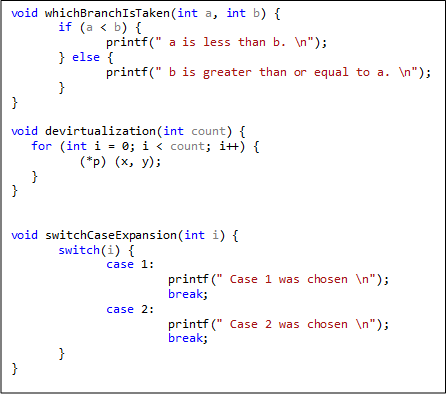
\includegraphics[width=0.5\textwidth]{images/4621codesnippet.png}
\end{center}

Just looking at this, which is more likely, \texttt{a < b} or \texttt{a >= b}? Assuming there's no other information in the system the compiler can believe that one is more likely than the other, or having no real information, use a fallback rule. This works, but what if we are wrong? Suppose the compiler decides it is likely that \texttt{a} is the larger value and it optimizes for that version. However, it is only the case 5\% of the time, so most of the time the prediction is wrong. That's unpleasant. But the only way to know is to actually run the program.

There are similar questions raised for the other two examples. What is the ``normal'' value for some pointer \texttt{p}? If we do not know, the compiler cannot do devirtualization (replace this virtual call with a real one). Same thing with \texttt{i}: what is its typical value? If we know that, it is our prediction. Actually, in a switch-case block with many options, could we rank them in descending order of likelihood?

There exists a solution to this, and it is that we can give hints to the compiler, but that's a manual process. Automation is a good thing and this lecture is about that. These sorts of things already exist for Java! The Java HotSpot virtual machine will update its predictions on the fly. There are some initial predictions and if they turn out to be wrong, the Just In Time compiler will replace it with the other version. That's neat! I don't know for certain but I suspect the .NET runtime will do the same for something like C\#. But this is C(++) (Sparta) and we don't have that: the compiler runs and it does its job and that's it; the program is never updated with newer predictions if more data becomes known.

Solving this problem is the goal of POGO. It is taking the data from some actual runs of the program and using that to inform the predictions. This necessitates a multi-step compile: first compile the code, run it to collect data, then recompile the code using the data we collected. Let's expand on all three steps.

Step one is to generate an executable with instrumentation. The compiler inserts a bunch of probes into the generated code that are used to record data. Three types of probe are inserted: function entry probes, edge probes, and value probes.  A function entry probe, obviously, counts how many times a particular function is called. An edge probe is used to count the transitions (which tells us whether an if branch is taken or the else condition). Value probes are interesting; they are used to collect a histogram of values. Thus, we can have a small table that tells us the frequency of what is given in to a \texttt{switch} statement. When this phase is complete, there is an instrumented executable and an empty database file where the training data goes~\cite{pogo}.

Step two is training day: run the instrumented executable through real-world scenarios. Ideally you will spend the training time on the performance-critical sections. It does not have to be a single training run, of course, data can be collected from as many runs as desired.   Still, it is important to note that you are not trying to exercise every part of the program (this is not unit testing); instead it should be as close to real-world-usage as can be accomplished. In fact, trying to use every bell and whistle of the program is counterproductive; if the usage data does not match real world scenarios then  the compiler has been given the wrong information about what is important. Or you might end up teaching it that almost nothing is important...

Step three is a recompile. This time, in addition to the source files, the training data is fed into the compiler for a second compile, and this data is applied to produce a better output executable than could be achieved by static analysis alone.

The Intel Developer Zone explains the process in a handy infographic\footnote{Source: \url{https://software.intel.com/en-us/node/522721}} :

\begin{center}
	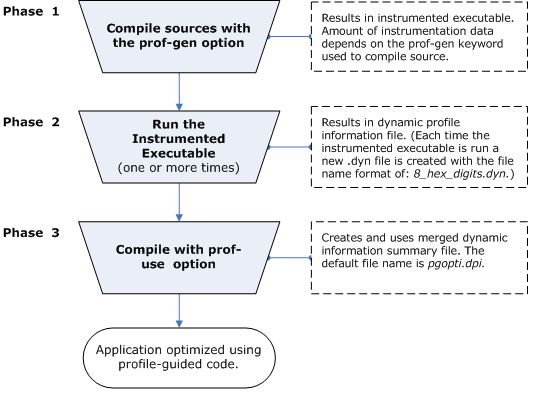
\includegraphics[width=0.5\textwidth]{images/pogo-workflow.jpg}
\end{center}

It is not necessary to do all three steps for every build. Old training data can be re-used until the code base has diverged significantly enough from the instrumented version. According to~\cite{pogo}, the recommended workflow is for one developer to perform these steps and check the training data into source control so that other developers can make use of it in their builds.

What does it mean for it to be better? We have already looked at an example about how to predict branches. Predicting it correctly will be faster than predicting it incorrectly, but this is not the only thing.  The algorithms will aim for speed in the areas that are ``hot'' (performance critical and/or common scenarios). The algorithms will alternatively aim to minimize the size of code of areas that are ``cold'' (not heavily used). It is recommended in~\cite{pogo} that less than 5\% of methods should be compiled for speed.

It is possible that we can combine multiple training runs and we can manually give some suggestions of what scenarios are important. Obviously the more a scenario runs in the training data, the more important it will be, as far as the POGO optimization routine is concerned, but multiple runs can be merged with user assigned weightings.

\subsection*{Behind the Scenes}

In the optimize phase, the training data is used to do the following optimizations~\cite{pogo2}:

\begin{multicols}{2}
\begin{enumerate}
\item Full and partial inlining
\item Function layout
\item Speed and size decision
\item Basic block layout 
\item Code separation
\item Virtual call speculation
\item Switch expansion
\item Data separation
\item Loop unrolling
\end{enumerate}
\end{multicols}

For the most part we should be familiar with the techniques that are listed as being other compiler optimizations we have previously discussed. The new ones are (3) speed and size decision, which we have just covered; and items (4) and (5) which relate to how to pack the generated code in the binary.

According to~\cite{pogo2} the majority of the performance gains relate to the inlining decisions. These decisions are based on the call graph path profiling: the behaviour of function \texttt{foo} may be very different when calling it from \texttt{bar} than it is when calling it from function \texttt{baz}\footnote{Why are these the example function names?! It's kind of like Alice and Bob...}. Great, let's look at this call graph from~\cite{pogo2}:

\begin{center}
	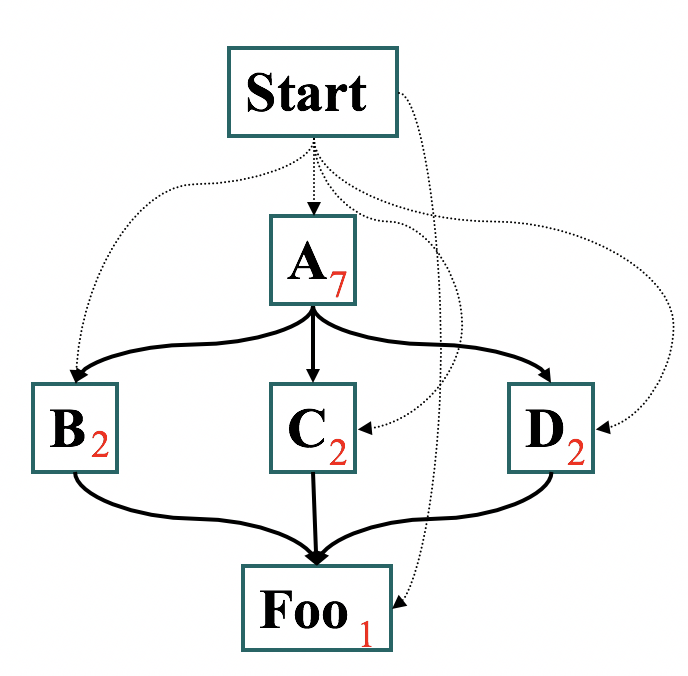
\includegraphics[width=0.25\textwidth]{images/callpaths.png}
\end{center}

Quick analysis of this code would have us find all the ways in which the functions might call each other. In total, there are 14 paths in this code, seven of which get us to function \texttt{Foo}.  

Consider another diagram showing the relationships between functions, in which the numbers on the edges represent the number of invocations~\cite{pogo2}:

\begin{center}
	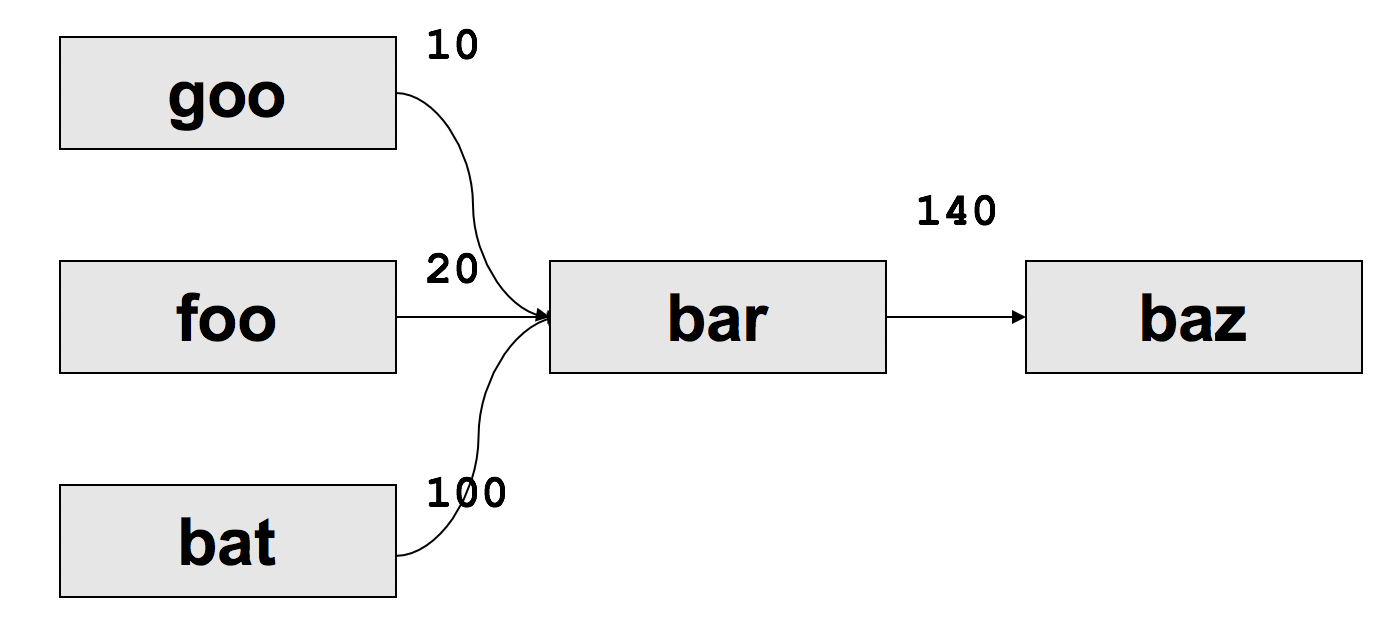
\includegraphics[width=0.4\textwidth]{images/callpaths2.png}
\end{center}

When considering what to do here, POGO takes the view like this~\cite{pogo2}:

\begin{center}
	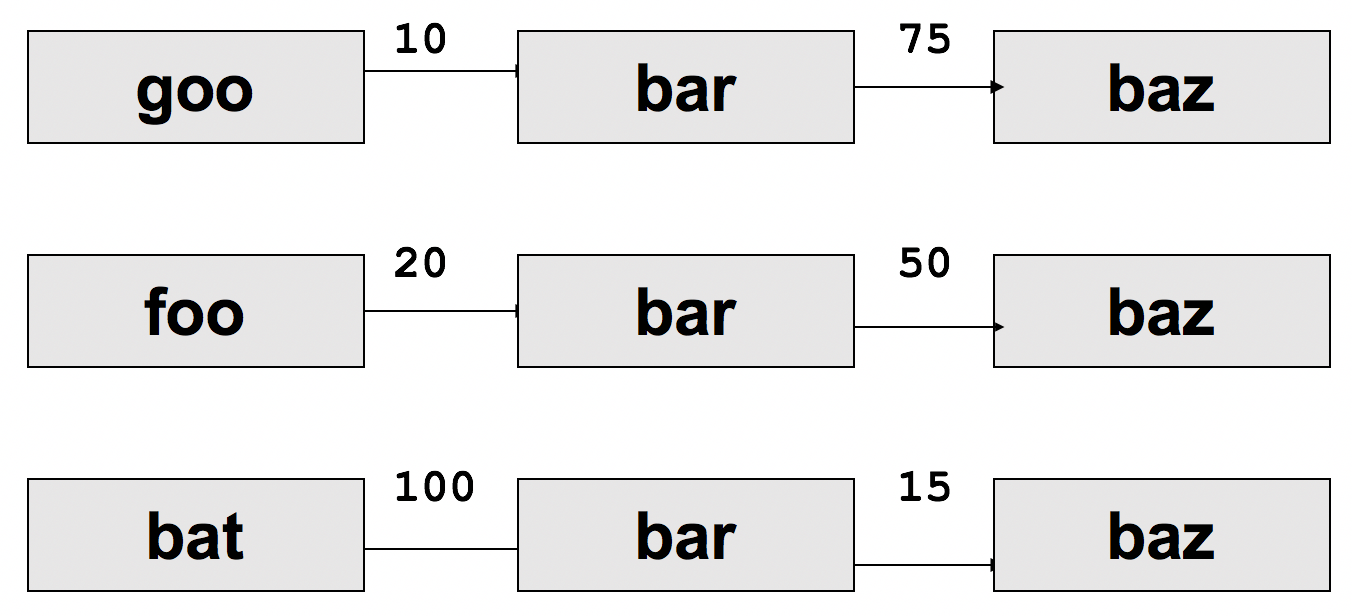
\includegraphics[width=0.4\textwidth]{images/callpaths3.png}
\end{center}

Each part of the call path is considered separately, remembering that we want to inline where it makes sense for speed, but otherwise leave it alone because of code size increases. Inlining \texttt{bar} into \texttt{bat} makes sense, but not inlining \texttt{bar} into \texttt{goo} (because that increases the code size without significant performance benefits). It also makes sense for \texttt{baz} to get inlined into \texttt{bar}. This is illustrated below~\cite{pogo2}:

\begin{center}
	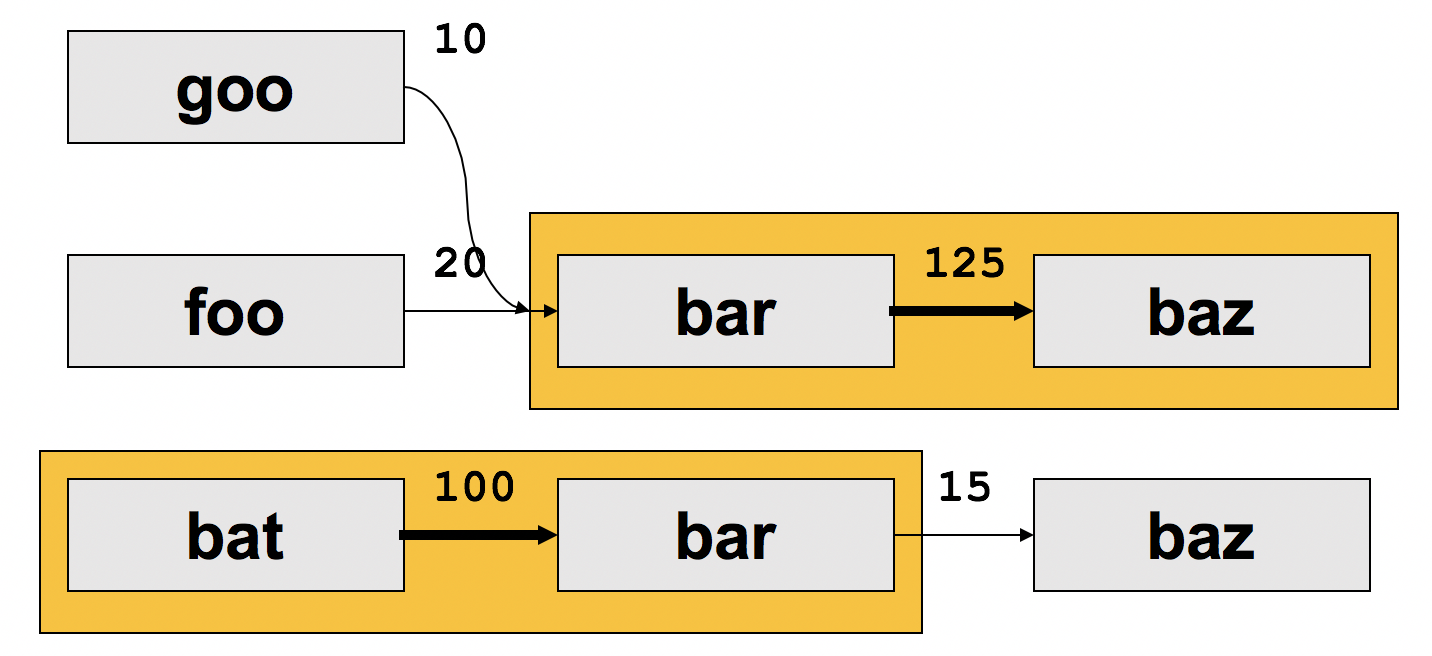
\includegraphics[width=0.4\textwidth]{images/callpaths4.png}
\end{center}

Packing the blocks is also done based on this call graph profiling. The most common cases will be put next to each other, and, where possible, subsequent steps are put next to each other. The more we can pack related code together, the fewer page faults we get by jumping to some other section, causing a cache miss... If the function being called is in the same page as the call, it has achieved ``page locality'' (and that is the goal!). This is represented visually~\cite{pogo2}:

\begin{center}
	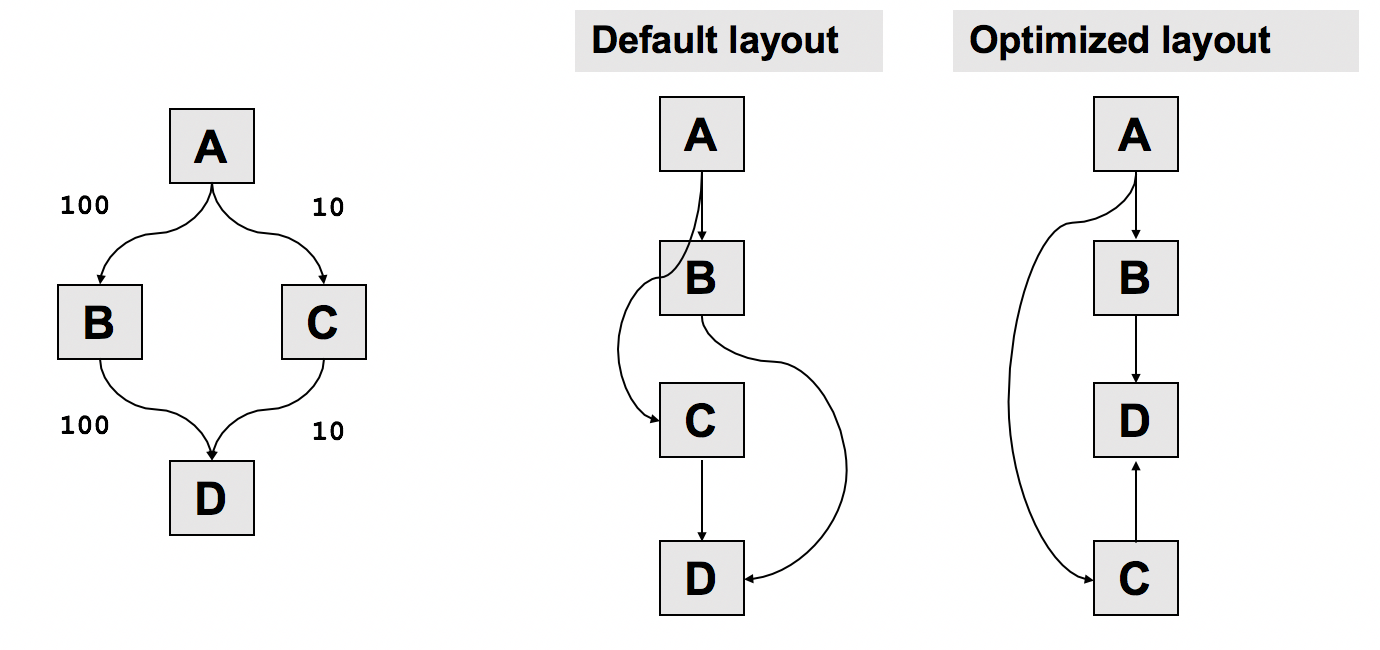
\includegraphics[width=0.6\textwidth]{images/blocklayout.png}
\end{center}

According to the author, the ``dead'' code goes in its own special block. I don't think they actually mean truly dead code, the kind that is compile-time determined to be unreachable, but instead they mean code that never gets invoked in any of the training runs.

So, to sum up, the training data is used to identify what branches are likely to be taken, inlines code where that is a performance increase, and tries to pack the binary code in such a way as to reduce cache misses/page faults. How well does it work?

\subsection*{Benchmark Results}

This table, condensed from~\cite{pogo2} summarizes the gains to be made. The application under test is a standard benchmark suite (Spec2K):

\begin{center}
\begin{tabular}{l|l|l|l|l|l}
	\textbf{Spec2k:} & \textbf{sjeng} & \textbf{gobmk} & \textbf{perl} & \textbf{povray} & \textbf{gcc}\\ \hline
	\textbf{App Size:} &  {Small} & {Medium} & {Medium} & {Medium} & {Large} \\ \hline
	\textbf{Inlined Edge Count} & 50\% & 53\% & 25\% & 79\% & 65\% \\ \hline
	\textbf{Page Locality} & 97\% & 75\% & 85\% & 98\% & 80\% \\ \hline
	\textbf{Speed Gain} & 8.5\% & 6.6\% & 14.9\% & 36.9\% & 7.9\% \\ 
\end{tabular}
\end{center}

There are more details in the source as to how many functions are used in a typical run and how many things were inlined and so on. But we get enough of an idea from the last row of how much we are speeding up the program, plus some information about why. We can speculate about how well the results in a synthetic benchmark translate to real-world application performance, but at least from this view it does seem to be a net gain.



\bibliographystyle{alphaurl}
\bibliography{459}



\end{document}
